\documentclass[aspectratio=169, table]{beamer}
\usepackage[utf8]{inputenc}
\usepackage[T1]{fontenc}
\usepackage{graphicx}
\usepackage{fontspec}
\usepackage{xcolor}
\usepackage{tcolorbox}
\usepackage{listings} % Add the listings package
\usepackage{hyperref} % Add the hyperref package

\lstdefinelanguage{JavaScript}{
    keywords={function, var, let, const, if, else, for, while, return, true, false},
    keywordstyle=\color{blue}\bfseries,
    ndkeywords={class, export, boolean, throw, implements, import, this},
    ndkeywordstyle=\color{orange}\bfseries,
    identifierstyle=\color{black},
    sensitive=false,
    comment=[l]{//},
    morecomment=[s]{/*}{*/},
    commentstyle=\color{gray}\ttfamily,
    stringstyle=\color{green}\ttfamily,
}

\lstset{
    breaklines=true,
    language=JavaScript,
    % ... (other style settings)
}

\setsansfont[
  ItalicFont=fonts/TitilliumWeb-Italic.ttf,
  BoldFont=fonts/TitilliumWeb-Bold.ttf,
  BoldItalicFont=fonts/TitilliumWeb-BoldItalic.ttf,
]{TitilliumWeb-Regular.ttf}

\subtitle{IF120203-Web Programming}
\title{\huge {\textbf{05: Introduction to\\Bootstrap, Grid, and Flex}}}
\date[Serial]{\scriptsize {PRU/SPMI/FR-BM-18/0222}}
\author[Pradita]{\small {\textbf{PRADITA UNIVERSITY}}}

\usetheme{Pradita}

\begin{document}
\begin{frame}
    \titlepage
\end{frame}

\begin{frame}{Goals for Today}
    \vskip-1cm
    \begin{itemize}
        \item To learn about the basic of Bootstrap
        \item To be able to understand how bootstrap as a CSS Framework works
        \item To understand how grid and flex works for web development
        \item To know when to apply flex or grid in any cases
    \end{itemize}
\end{frame}

\begin{frame}{Introduction to Bootstrap}
    \vskip-0cm
    \begin{itemize}
        \item Bootstrap is a free and open-source CSS framework directed at responsive, mobile-first front-end web development.
        \item Bootstrap makes responsive web design a reality. It makes it possible for a web page or app to detect the visitor's screen size and orientation and automatically adapt the display accordingly.
    \end{itemize}
\end{frame}

\begin{frame}[fragile]
	\frametitle{Example: Button - CSS Native}
	\vskip1cm
	\begin{center}
		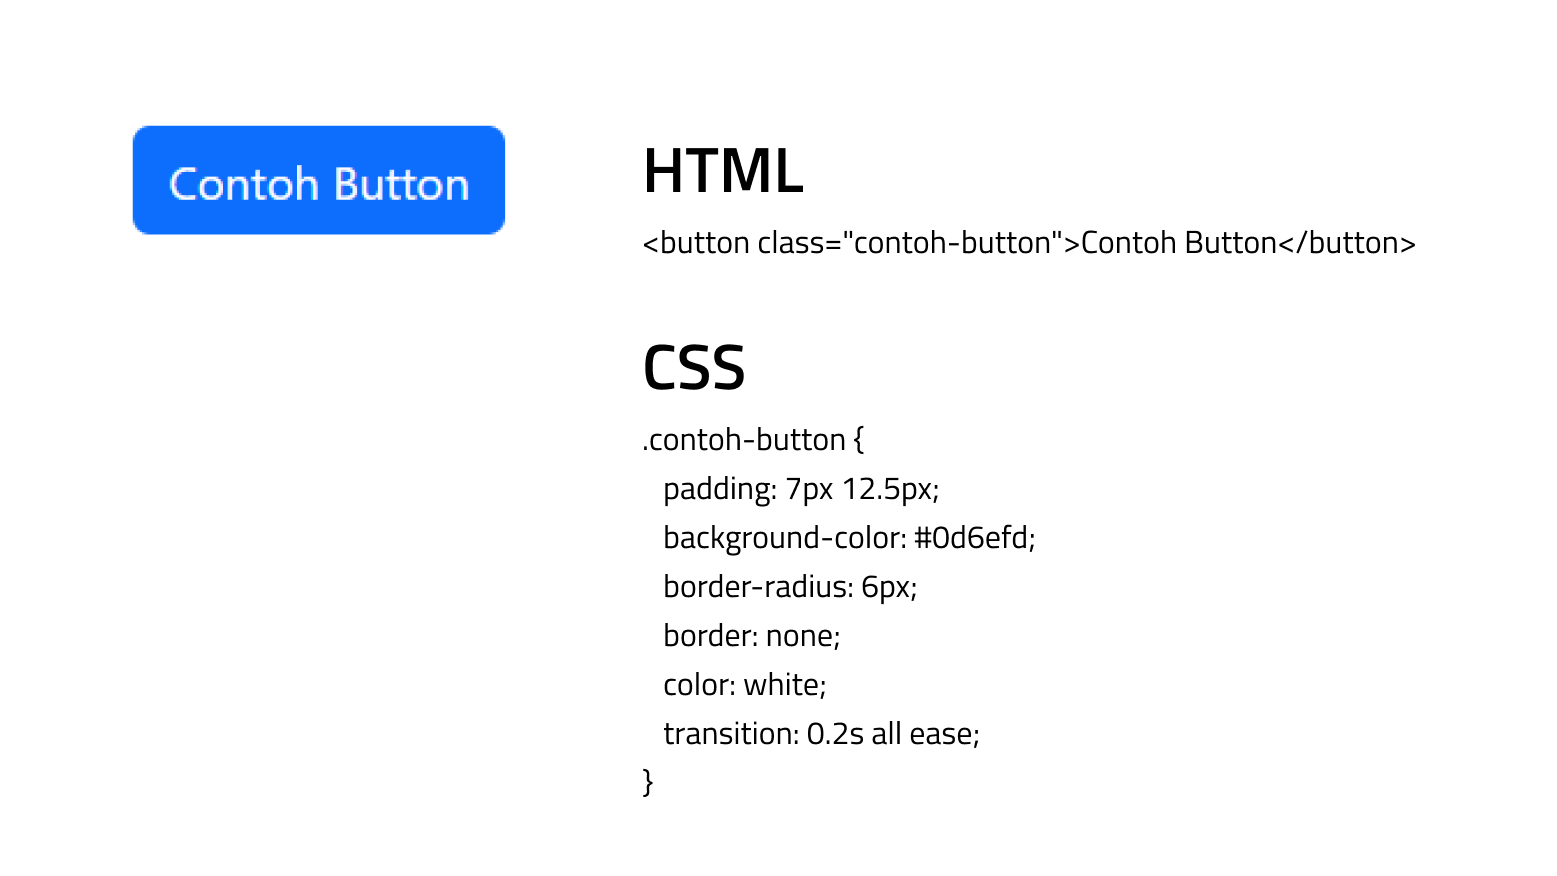
\includegraphics[width=0.8\textwidth]{classFiles/button-css-native.png}
	\end{center}
\end{frame}

\begin{frame}[fragile]
	\frametitle{Example: Button - Bootstrap}
	\vskip1cm
	\begin{center}
		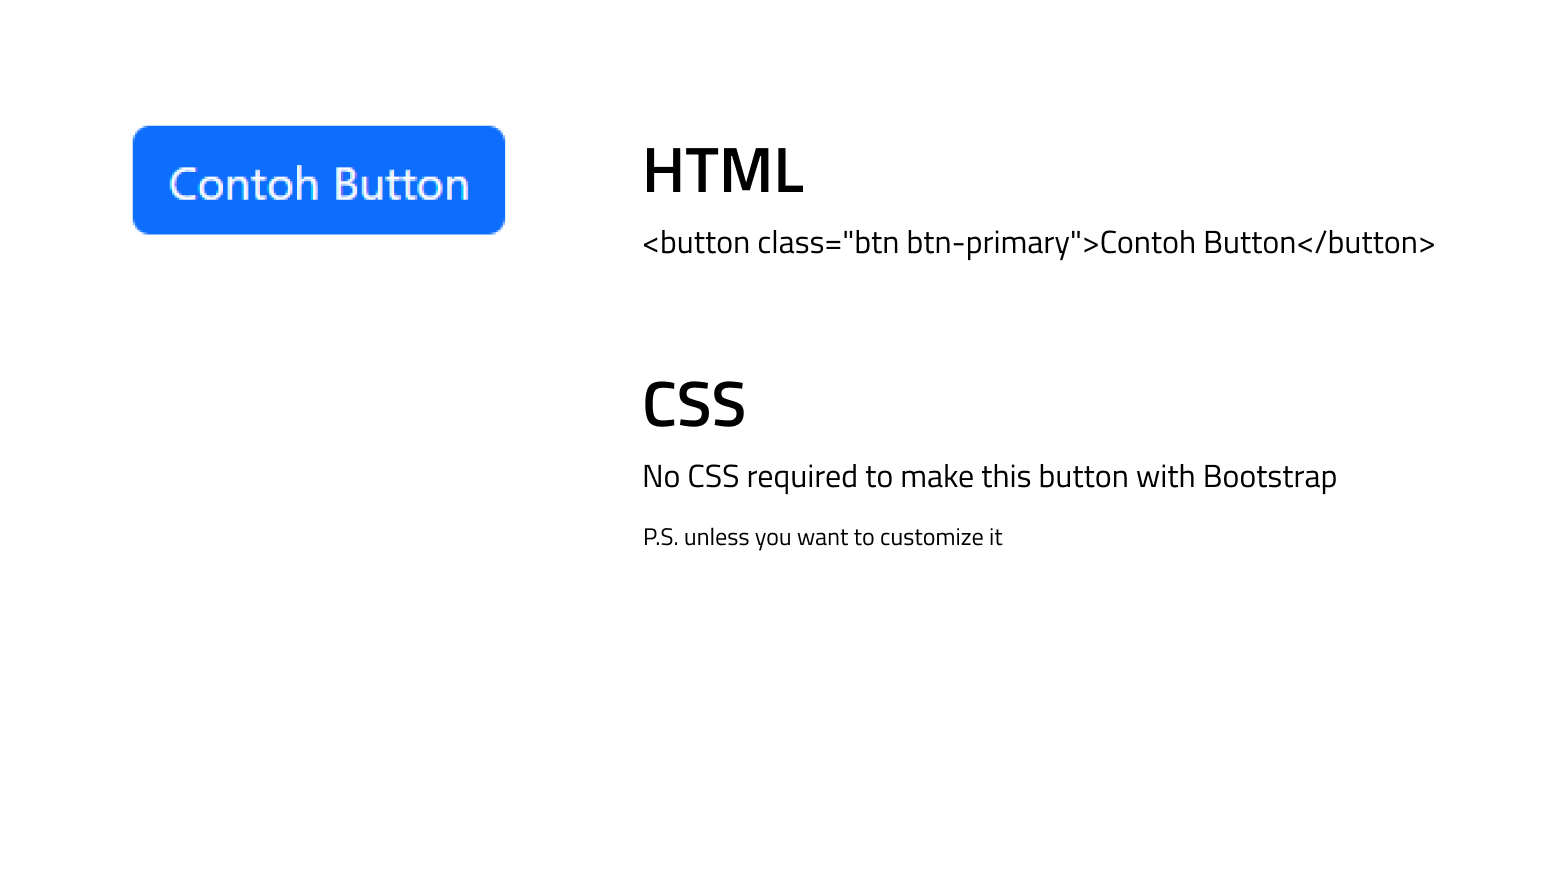
\includegraphics[width=0.8\textwidth]{classFiles/button-bootstrap.png}
	\end{center}
\end{frame}


% ... (previous frames)

\begin{frame2}
   \frametitle{Benefit of using Bootstrap}
   \vskip1cm
    \begin{itemize}
        \item A consistent framework that supports major of all browsers \\and CSS compatibility fixes
        \item Lightweight and customizable
        \item Responsive structures and styles
	\item Good documentation and community support
    \end{itemize}
\end{frame2}

\begin{frame2}
    \frametitle{Introduction to Grid}
    \vskip2cm
    \begin{itemize}
        \item Grid in CSS is a layout technique that divides a webpage into\\ rows and columns, creating a structured grid structure. 
        \item Grid in CSS is a powerful layout system that simplifies the way \\we arrange elements on a web page. When paired with \\frameworks like Bootstrap, it becomes even more \\accessible and efficient. 
        \item Instead of relying solely on float-based layouts or complex\\ positioning, Grid offers a straightforward and intuitive way to \\manage page structure.
    \end{itemize}
\end{frame2}

\begin{frame}
    \frametitle{Introduction to Grid}
    \vskip1cm
    \begin{itemize}
        \item Grid in Bootstrap is a size setting that is displayed on the monitor. Grid Bootstrap functions to make settings for the width of each web component so that we can freely adjust the responsiveness of the website pages that we create with Bootstrap. Bootstrap has 12 grid classes.
    \end{itemize}
    \begin{center}
	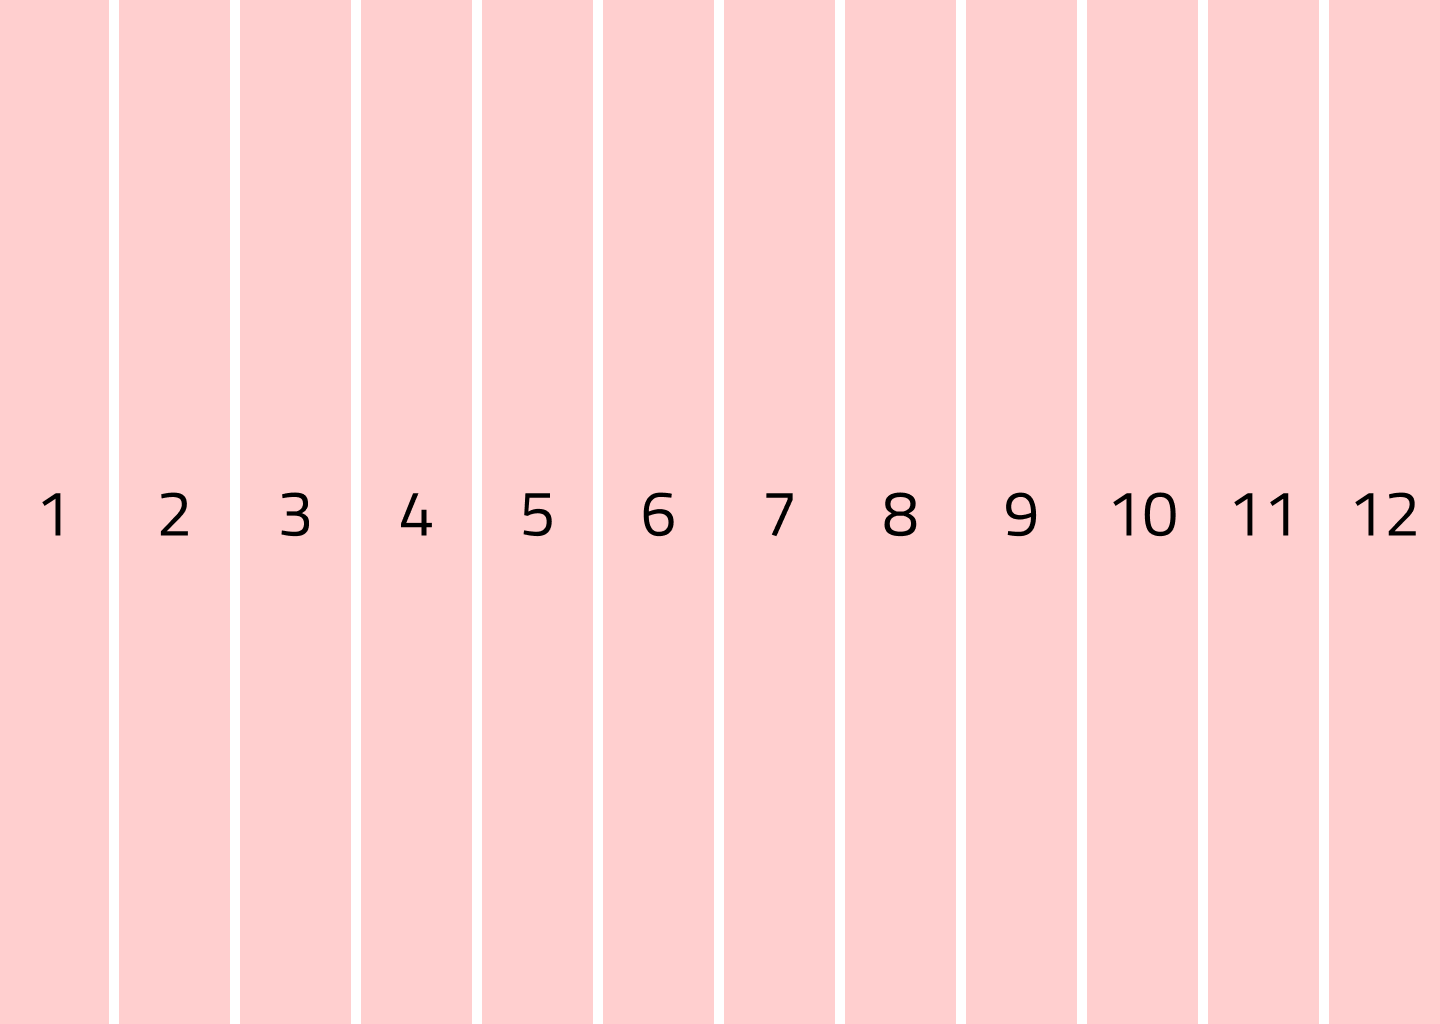
\includegraphics[width=0.4\textwidth]{classFiles/grid-general.jpg}
    \end{center}
\end{frame}


\begin{frame}
    \frametitle{Grid Customization - 1}
    \vskip0cm
    \begin{itemize}
        \item Bootstrap's grid system is based on a 12-column layout, where the screen width is divided into 12 equal parts. This provides a convenient way to create responsive designs that adapt to different screen sizes. Each column is represented by a class, typically named col-*, where the * is a number from 1 to 12.
	\item When designing your layout, you can use these column classes to define the width of each column within a row. For example, col-6 means the column occupies half the width of the row, while col-3 means the column takes up one-fourth of the row's width.
    \end{itemize}
\end{frame}

\begin{frame}
    \frametitle{Grid Customization - 2}
    \vskip1cm
    \begin{itemize}
        \item If the total column count in a row exceeds 12, Bootstrap's grid system will automatically wrap the overflowing columns onto the next line. This ensures that your content remains visually coherent and doesn't break the layout. Here's how this works:
	\item 1. Overflowing Columns: Let's say you have a row with columns col-6, col-4, col-3, and col-2. The total column count is 6 + 4 + 3 + 2 = 15, which exceeds 12.
	\item 2. Automatic Wrapping: In this scenario, Bootstrap will wrap the overflowing columns to the next line while maintaining the column order. So, the first row will contain columns col-6 and col-4, and the second row will have columns col-3 and col-2.
    \end{itemize}
\end{frame}

\begin{frame}
    \frametitle{Grid Visualization}
    \vskip1cm
    \begin{center}
	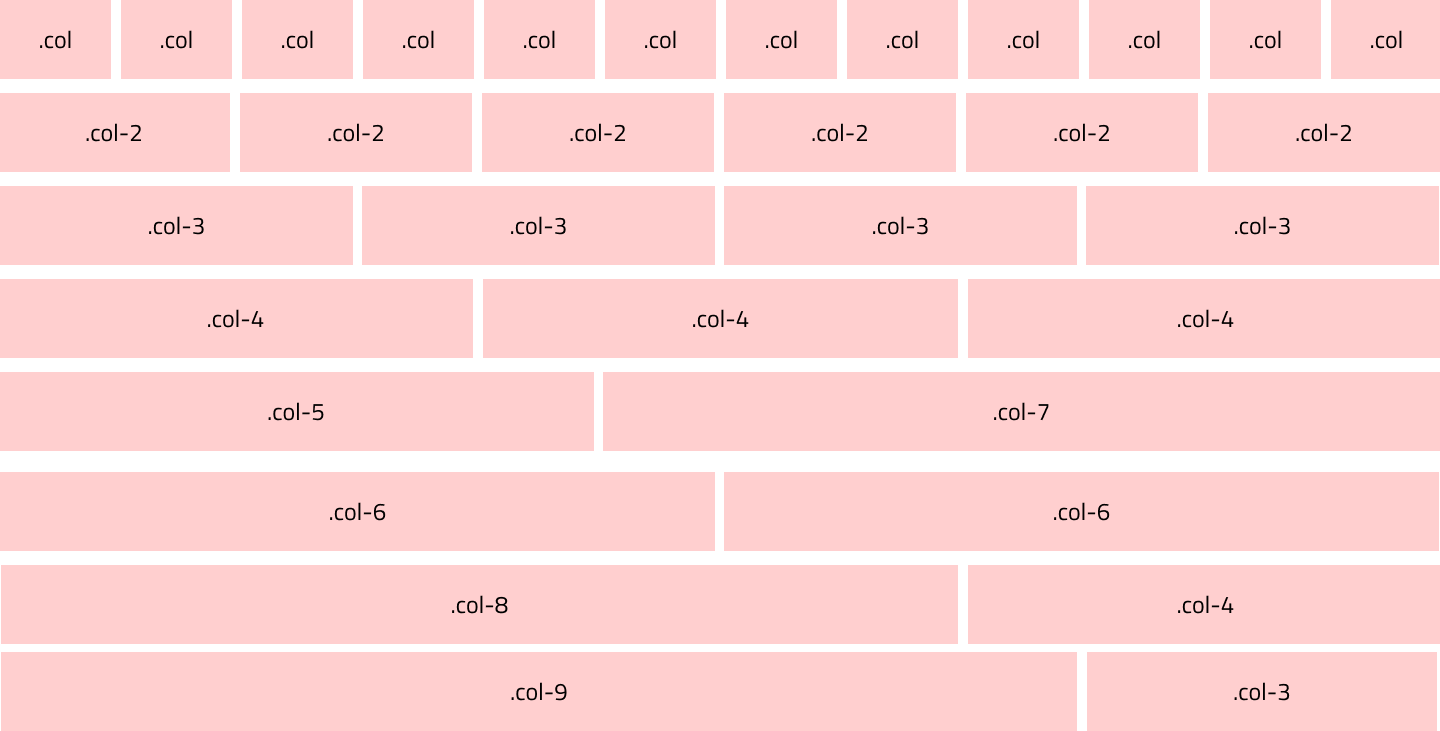
\includegraphics[width=0.8\textwidth]{classFiles/grid-custom.png}
    \end{center}
\end{frame}

\begin{frame3}
    \vskip1cm
    \begin{tcolorbox}[standard jigsaw, opacityback=0, opacityframe=0, sharp corners, boxrule=0pt]
        \begin{columns}[T] %T for Top, C for Center, B for Bottom
            \begin{column}{0.5\textwidth}	
		\textbf{\huge{\textcolor{white}{Introduction to Flex - 1\\}}}
                \textbf{\textcolor{white}{\\Flexbox, short for Flexible Box Layout, is a CSS layout model designed to provide an efficient way to arrange and distribute space among items in a container, even when their sizes are unknown or dynamic. Flexbox is particularly well-suited for creating complex layouts and aligning items within a container in a more predictable and consistent manner.}}
            \end{column}
            \begin{column}{0.5\textwidth}
		\begin{center}
                	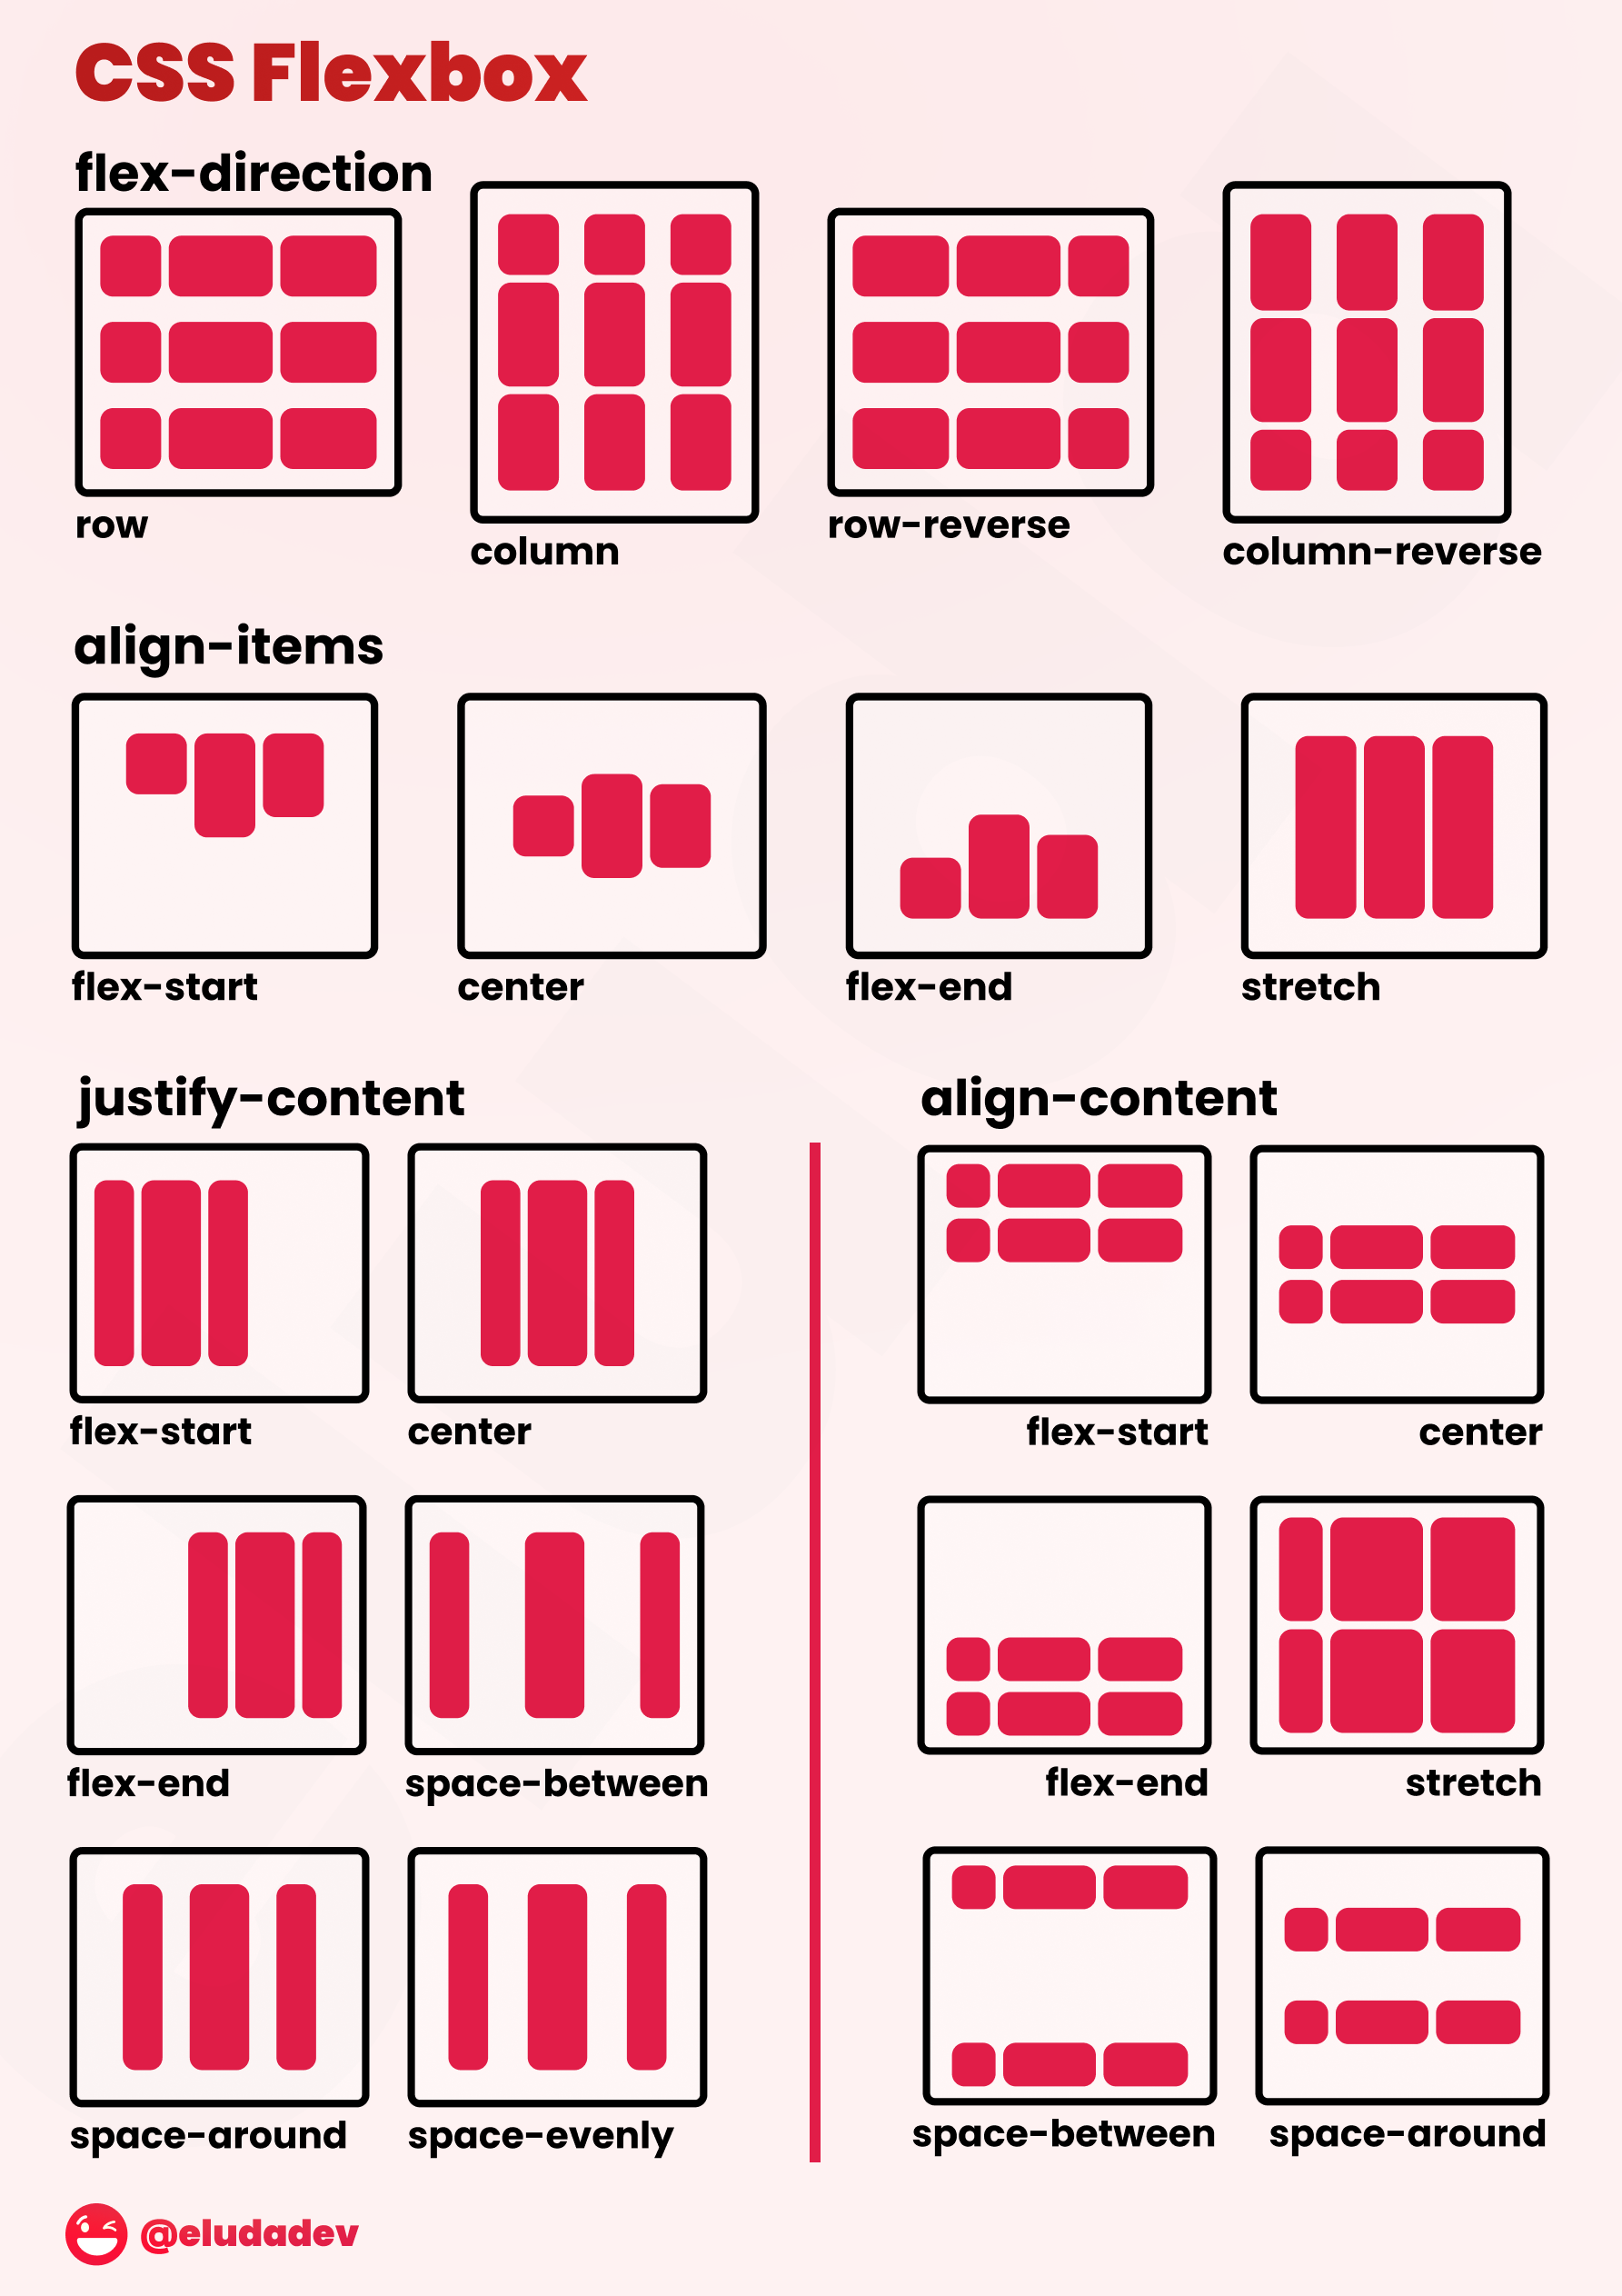
\includegraphics[width=0.7\textwidth]{classFiles/flexbox-guideline.png}
		\end{center}
            \end{column}
        \end{columns}
    \end{tcolorbox}
\end{frame3}

\begin{frame}
    \frametitle{Introduction of Flex - 2}
    \vskip1cm
    \begin{itemize}
        \item In the Flexbox model, you work with two main components: the flex container and the flex items.
	\item 1. Flex Container: The parent element that holds the flex items. To create a flex container, you apply the display: flex; or display: inline-flex; property to the container element. This establishes a new flex formatting context for the container and its direct children become flex items.
	\item 2. Flex Items: The child elements of the flex container. These items can be arranged horizontally (in a row) or vertically (in a column). Flex items can grow, shrink, and be aligned based on various properties.
    \end{itemize}
\end{frame}

\begin{frame}
    \frametitle{Introduction of Flex - 3}
    \vskip1cm
    \begin{itemize}
        \item flex-direction: This property defines the main axis along which the flex items will be placed. The values can be row (default), row-reverse, column, or column-reverse.
	\item justify-content: This property aligns flex items along the main axis. When the flex-direction is set to row, it controls horizontal alignment, and when set to column, it controls vertical alignment. Common values include flex-start, flex-end, center, space-between, and space-around.
	\item align-items: This property aligns flex items along the cross axis (the axis perpendicular to the main axis). When the flex-direction is row, it controls vertical alignment, and when set to column, it controls horizontal alignment. Common values include flex-start, flex-end, center, baseline, and stretch.
    \end{itemize}
\end{frame}

\begin{frame}
    \frametitle{Introduction of Flex - 4}
    \vskip1cm
    \begin{itemize}
        \item When you change the flex-direction to column, the behavior of justify-content and align-items switches because the main axis and cross axis orientations change:
	\item With flex-direction: column, the main axis becomes vertical and the cross axis becomes horizontal.
	\item justify-content now controls vertical alignment, similar to how align-items worked in the row direction. It aligns flex items vertically within the column.
	\item align-items now controls horizontal alignment, similar to how justify-content worked in the row direction. It aligns flex items horizontally within the column.
    \end{itemize}
\end{frame}




\begin{frame}[fragile]
    \frametitle{JQuery Reverse Button}
    \begin{lstlisting}[language=JavaScript]
$(document).ready(function () {
  $("#reverse").click(function () {
    const fromSelect = $("#from");
    const toSelect = $("#to");
    const temp = fromSelect.val();
    fromSelect.val(toSelect.val());
    toSelect.val(temp);
  });
// Next is Convert Button
    \end{lstlisting}
\end{frame}

\begin{frame}[fragile]
    \frametitle{JQuery Convert Button - Part 1}
    \begin{lstlisting}[language=JavaScript]
  $("#convert").click(async function () {
    const fromSelect = $("#from");
    const toSelect = $("#to");
    const apiKey = "fca_live_iq1WvbaON67X9adHTaJiqEszDhP6jtDz7IouUbWv";
    const fromCurrency = fromSelect.val();
    const toCurrency = toSelect.val();
    \end{lstlisting}
\end{frame}

\begin{frame}[fragile]
    \frametitle{JQuery Convert Button - Part 2}
    \begin{lstlisting}[language=JavaScript]
const encodedFromCurrency = encodeURIComponent(fromCurrency);
    const encodedToCurrency = encodeURIComponent(toCurrency);

    const url = `https://api.freecurrencyapi.com/v1/latest?apikey=${apiKey}&currencies=${encodedToCurrency}&base_currency=${encodedFromCurrency}`;
    const options = {
      method: "GET",
    };
    \end{lstlisting}
\end{frame}

\begin{frame}[fragile]
    \frametitle{JQuery Convert Button - Part 3}
    \begin{lstlisting}[language=JavaScript]
try {
      const response = await fetch(url, options);
      const data = await response.json(); // Parse the response body as JSON
      // console.log(data); // For debugging purposes
      const rate = data["data"][toSelect.val()]; // Get the rate value for the selected currency
      const amount = $("#amount").val();
      const converted = (amount * rate).toLocaleString(undefined, {
        minimumFractionDigits: 2,
        maximumFractionDigits: 2,
      });
    \end{lstlisting}
\end{frame}

\begin{frame}[fragile]
    \frametitle{JQuery Convert Button - Part 4}
    \begin{lstlisting}[language=JavaScript]
let fromCurrencySymbol;
      if (fromSelect.val() === "IDR") {
        fromCurrencySymbol = "Rp. ";
      } else if (fromSelect.val() === "USD") {
        fromCurrencySymbol = "$ ";
      } else if (fromSelect.val() === "EUR") {
        fromCurrencySymbol = "€ ";
      } else if (fromSelect.val() === "GBP") {
        fromCurrencySymbol = "£ ";
      }
    \end{lstlisting}
\end{frame}

\begin{frame}[fragile]
    \frametitle{JQuery Convert Button - Part 5}
    \begin{lstlisting}[language=JavaScript]
let toCurrencySymbol;
      if (toSelect.val() === "IDR") {
        toCurrencySymbol = "Rp. ";
      } else if (toSelect.val() === "USD") {
        toCurrencySymbol = "$ ";
      } else if (toSelect.val() === "EUR") {
        toCurrencySymbol = "€ ";
      } else if (toSelect.val() === "GBP") {
        toCurrencySymbol = "£ ";
      }
    \end{lstlisting}
\end{frame}

\begin{frame}[fragile]
    \frametitle{JQuery Convert Button - Part 6}
    \begin{lstlisting}[language=JavaScript]
$("#from-result").text(fromCurrencySymbol + amount);
      $("#from-currency").text(fromSelect.val());
      $("#to-result").text(toCurrencySymbol + converted);
      $("#to-currency").text(toSelect.val());
      const exchangeRateLabel = $("#exchange-rate");
      const formattedRate = parseFloat(rate).toFixed(2);
      const exchangeRateText = `1 ${fromSelect.val()} = ${formattedRate} ${toSelect.val()}`;
    \end{lstlisting}
\end{frame}

\begin{frame}[fragile]
    \frametitle{JQuery Convert Button - Part 7}
    \begin{lstlisting}[language=JavaScript]
      exchangeRateLabel.text(exchangeRateText);
    } catch (error) {
      console.error(error);
    }
  });
});
    \end{lstlisting}
\end{frame}

\begin{frame4}
    \frametitle{Thank You}
\end{frame4}

\end{document}
